\documentclass[12pt, a4paper]{article}

\usepackage{amsmath}
\usepackage{bm}
\usepackage{array}
\usepackage{amsmath}
\usepackage[portuguese]{babel}
\usepackage{chngpage}
\usepackage{float}
\usepackage[a4paper, margin=2cm]{geometry}
\usepackage{graphicx}
\usepackage{hyperref}
\usepackage{listings}
\usepackage{setspace}
\usepackage{tikz}
\usepackage{xcolor}

\usetikzlibrary{arrows, arrows.meta}

\lstdefinestyle{codestyle}{
    commentstyle=\color{teal},
    keywordstyle=\color{blue},
    numberstyle=\ttfamily\color{gray},
    stringstyle=\color{red},
    basicstyle=\ttfamily\footnotesize,
    breakatwhitespace=false,
    breaklines=false,
    keepspaces=true,
    numbers=none,
    showspaces=false,
    showstringspaces=false,
    showtabs=false,
    tabsize=4
}
\lstset{style=codestyle}

\title{\Huge \textbf{Computação Gráfica \\ \Large Trabalho Prático -- Fase III}}
\date{27 de abril de 2025}
\author{Grupo 3}

\begin{document}

\begin{center}
    
\includegraphics[width=0.25\textwidth]{res/cover/EE-C.eps}
\end{center}

\chardef\_=`_
\onehalfspacing
\setlength{\parskip}{\baselineskip}
\setlength{\parindent}{0pt}
\def\arraystretch{1.5}

{\let\newpage\relax\maketitle}
\maketitle
\thispagestyle{empty}

\vspace*{\fill}

\begin{adjustwidth}{-2cm}{-2cm} % These values only need to be large enough to center the table
    \begin{center}
        \begin{tabular}{>{\centering}p{0.25\textwidth}
                        >{\centering}p{0.25\textwidth}
                        >{\centering}p{0.25\textwidth}
                        >{\centering\arraybackslash}p{0.25\textwidth}}
            
\includegraphics[width=3.5cm]{res/cover/A104437.png} &
            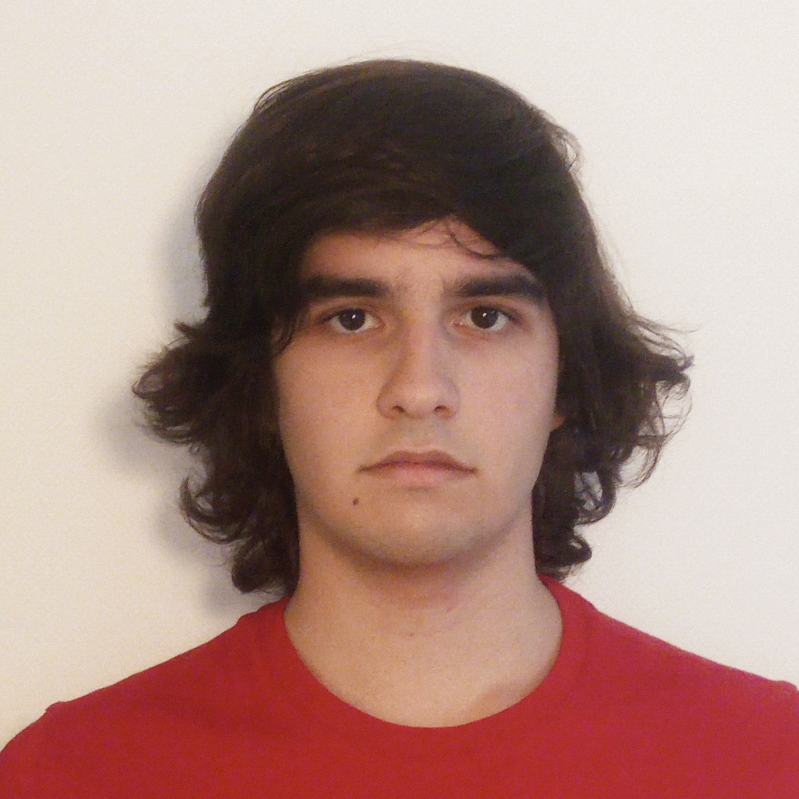
\includegraphics[width=3.5cm]{res/cover/A104348.png} &
            
\includegraphics[width=3.5cm]{res/cover/A90817.png} &
            
\includegraphics[width=3.5cm]{res/cover/A104179.png} \\

            Ana Oliveira & Humberto Gomes & Mariana Cristino & Sara Lopes \\
            A104437      & A104348        & A90817           & A104179
        \end{tabular}
    \end{center}
\end{adjustwidth}

\pagebreak

\begin{abstract}
{\color{red} TODO }
\end{abstract}

\section{\emph{Generator}}

Nesta fase, o código do programa \texttt{generator} passou por um processo de limpeza, para o tornar
mais consistente, melhorar a sua legibilidade, e corrigir algumas falhas nas quais não se tinha
reparado em fases anteriores. Ademais, nesta fase, foi implementada a geração de modelos 3D com base
em \emph{patches} de Bézier.

\subsection{Alterações à geração de figuras geométricas}

Em primeiro lugar, comece-se por mencionar o que não precisou de ser alterado. O \texttt{generator}
exporta os modelos 3D que gera no formato Wavefront OBJ \cite{wavefront-obj}, que foi descrito em
detalhe no relatório da primeira fase deste trabalho prático. Em suma, este formato consiste numa
sequência de vértices seguida de um conjunto de faces triangulares, e estas faces são definidas com
índices de vértices da sequência mencionada. Logo, já desde a primeira fase, a \texttt{engine} tira
proveito desta indexação no formato Wavefront OBJ para indexar os vértices dos modelos carregados
para a GPU, não tendo sido necessária qualquer alteração ao \texttt{generator} para gerar modelos
mais pequenos e que tiram proveito da \emph{cache} de vértices da GPU.

% TODO - Ver se adicionar os vértices tem algum benefício. Eu desliguei o V-Sync, a UI, aumentei o
%        número de slices e de stacks, e não observei nenhuma diferença entre entre o generator
%        antigo e o novo. É melhor falar na aula e, se não houver qualquer diferença teórica / for
%        negligenciável, nem falamos disto no relatório, já que foi só mudar uns <=.

% No entanto, anteriormente, em alguns modelos gerados, a ordem dos vértices não originava padrões
% de acesso à memória ideais, o que se procurou resolver nesta fase do trabalho.

% Alguns sólidos de revolução, em específico, a esfera, o cone, e o cilindro, são desenhados
% \emph{stack} a \emph{stack}, ou seja, com base em cada duas \emph{stacks}, desenha-se uma fita de
% quadriláteros, cada um dividido em dois triângulos. Anteriormente, os últimos triângulos destas
% fitas reutilizavam os pontos da primeira \emph{slice}, levando a padrões de acesso a memória
% indesejáveis. A alteração que foi feita ao \texttt{generator} para mitigar este problema foi a
% duplicação dos vértices da primeira \emph{slice}. Deste modo, apesar dos modelos gerados ocuparem
% ligeiramente mais memória, apresentam melhores padrões de acesso a memória que podem conduzir a um
% melhor desempenho.

% {\color{red} TODO - figuras caso se coloque isto no relatório }

No entanto, é de notar que a geração de grelhas, presente em todas as figuras geradas, ainda podia
ser melhor otimizada para a \emph{cache} de vértices. Alguns métodos de indexação
\cite{optimal-grid} dão origem a modelos que são capazes de tirar um maior proveito da \emph{cache}
de vértices. No entanto, estes são um pouco mais complexos e envolvem a geração de triângulos
degenerados, pelo que se optou por não os utilizar, optando-se então por uma solução simples e fácil
de compreender.

Uma alteração ao processo de geração de modelos 3D foi a adição, a cada modelo, de um comentário que
enuncia os parâmetros utilizados na sua geração. Um exemplo de um destes comentários seria:

\begin{center}
\texttt{\# cone 1.000000 2.000000 4 2}
\end{center}

Ademais, o \emph{parser} de ficheiros Wavefront OBJ foi reimplementado com base em expressões
regulares, que o tornam mais eficiente e mais facilmente extensível. De momento, a única extensão
funcional em relação à fase anterior foi o suporte para comentários. No entanto, na próxima fase,
será necessário adicionar suporte para coordenadas de textura e vetores normais, e espera-se que o
uso de expressões regulares torne este processo mais fácil.

\subsection{Alterações à geração do Sistema Solar}

A geração do sistema solar também sofreu alterações. Em primeiro lugar, para simplificar o seu
código, as posições dos corpos celestes já não são especificadas manualmente, mas sim geradas de um
modo pseudo-aleatório: no código apenas se especifica a distância de um corpo ao seu pai, $d$, um
ângulo $\theta \in \left [ 0, 2\pi \right [$ é gerado aleatoriamente, e a posição do corpo é
calculada da seguinte forma:

$$
x = d \cos \theta
\hspace{1cm}
z = d \sin \theta
$$

Ademais, a parametrização da geração do Sistema Solar também foi alterada. Agora, são pedidos ao
utilizador menos argumentos, que permitem um controlo semelhante da aparência da cena gerada:

\begin{center}
\texttt{generator solarSystem [<sunScale> <rockyScale> <gasScale>] <directory>}
\end{center}

O utilizador agora pode, opcionalmente, definir a escala aplicada ao Sol (\texttt{sunScale}), aos
planetas rochosos e asteroides (\texttt{rockyScale}) e aos planetas gasosos (\texttt{gasScale}).
Também se observa que o \texttt{generator} passa a criar uma diretoria com vários ficheiros, em vez
de apenas um ficheiro com a cena. Os novos ficheiros criados são os modelos de uma esfera e de um
\emph{torus}, utilizados nos corpos celestes e nos seus anéis, respetivamente. Isto é uma melhoria
em relação à fase anterior, onde era esperado que o utilizador gerasse estes modelos manualmente.

De seguida, foi descoberto um problema com a estrutura hierárquica do Sistema Solar a ser gerada
anteriormente. Os objetos eram agrupados em grupos conforme a sua atração gravítica: corpos a
orbitar o Sol eram colocados no grupo do Sol, e corpos a orbitar um planeta eram colocados no grupo
desse planeta. Logo, todos os corpos a orbitar um corpo $X$ estariam sujeitos a todas as
transformações de $X$, quando apenas se deseja que estejam sujeitos à sua translação: se o Sol
sofrer uma rotação, não se deseja que os planetas rodem o mesmo ângulo (estejam
\emph{tidally locked}). Para resolver este problema, caso um corpo celeste tenha outros corpos a
orbitá-lo, é colocado num grupo aninhado no qual são colocadas as suas transformações de escala e de
rotação. Como exemplo, segue-se a estrutura da Terra e da Lua:

\lstset{language=xml}
\begin{lstlisting}

<group>
    <transform>
        <translate ... />
    </transform>
    <group>
        <transform>
            <scale ... />
            <rotate ... />
        </transform>
        <models>
            <model file="sphere.3d"/> <!-- Terra -->
        </models>
    </group>
    <group>
        <transform>
            <translate ... />
            <scale ... />
            <rotate ... />
        </transform>
        <models>
            <model file="sphere.3d"/> <!-- Lua -->
        </models>
    </group>
</group>
\end{lstlisting}

Como se pode observar, no grupo exterior encontra-se a translação aplicada tanto à Terra como à Lua.
A Terra, como é orbitada pela Lua, é colocada num grupo interior com a sua escala e rotação. Quanto
à Lua, como nada a orbita, no seu grupo encontram-se as suas três transformações.

Também houve uma alteração à hierarquia de grupos das cinturas de asteroides. Anteriormente, cada
asteroide era um grupo, e todos estes grupos tinham o mesmo pai. Isto não era ideal para o
\emph{frustum culling}, porque era necessário verificar para todo o asteroide se ele se encontrava
ou não no \emph{view frustum}. Seria possível evitar vários testes se um grupo contivesse vários
asteroides e a esfera encapsuladora desse grupo não fosse visível.

Logo, para resolver este problema, cada cintura de asteroides é divida em subgrupos. Para determinar
o tamanho de cada subgrupo, procura-se que o comprimento do arco a que está associado seja o mesmo
que a largura da cintura de asteroides. Deste modo, a esfera que encapsula os asteroides não será
nem pequena nem grande demais, o que levaria a um maior número de testes de \emph{frustum culling}.
Assim, dados os raios externo ($R$) e interno ($r$) de uma cintura de asteroides, o seu número de
grupos pode ser calculado do seguinte modo:

$$
N = \left \lceil \frac{2 \pi \cdot \frac{R + r}{2}}{R - r} \right \rceil
  = \left \lceil \frac{\pi (R + r)}{R - r} \right \rceil
$$

Essencialmente, esta fórmula calcula quantas vezes a largura da cintura de asteroides ($R - r$) cabe
no perímetro da sua circunferência média. Com esta divisão, as esferas encapsuladoras dos grupos de
uma cintura de asteroides são visíveis na figura abaixo.

\begin{figure}[H]
    \centering
    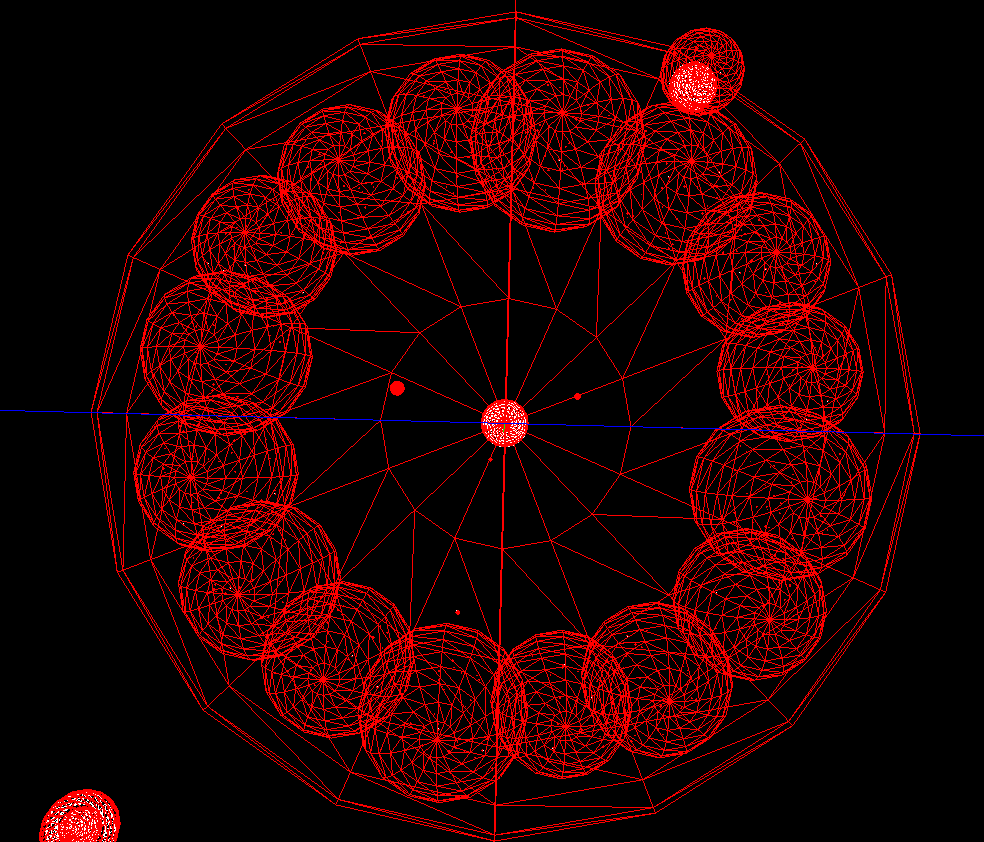
\includegraphics[width=0.5\textwidth]{res/phase3/AsteroidBeltBoundingSpheres.png}
    \caption{Esferas encapsuladoras dos grupos da cintura de asteroides interna.}
\end{figure}

{\color{red} TODO - falar de animações}

Por último, tal como foi feito com os modelos 3D, uma cena do Sistema Solar começa com um comentário
XML como o que pode ser visto abaixo, a enunciar os parâmetros com que foi gerada:

\begin{center}
    \texttt{<!-- solarSystem 1.000000 10.000000 10.000000 -->}
\end{center}

\subsection{Geração de modelos com base em \emph{patches} de Bézier}

Foi adicionada ao \texttt{generator} a funcionalidade de gerar modelos 3D com base em \emph{patches}
de Bézier e um nível de tesselação, o que pode ser feito com a linha de comando abaixo:

\begin{center}
    \texttt{generator bezier <patchFile> <tessellation> <file>}
\end{center}

Após o \emph{parsing} do ficheiro de \emph{patches}, é necessário agregar o conjunto de pontos
associado a cada \emph{patch} com base nos seus índices
($p_{i j}, i, j \in \left \lbrace 1,2,3,4 \right \rbrace$). Depois, é necessário calcular as
coordenadas dos pontos no \emph{patch}. Matematicamente, é necessário considerar em primeiro lugar
as seguintes matrizes, notando que, nas expressões abaixo, $c$ corresponde a uma coordenada, $x$,
$y$ ou $z$:

$$
\def\arraystretch{1}
M =
\begin{bmatrix}
    -1 &  3 & -3 & 1 \\
     3 & -6 &  3 & 0 \\
    -3 &  3 &  0 & 0 \\
     1 &  0 &  0 & 0
\end{bmatrix}
\hspace{1cm}
P_c = \left [ {p_{i j}}_{c} \right ] _ {4 \times 4}
$$

Depois, os pontos na superfície de um \emph{patch} são dados por:

$$
\def\arraystretch{1}
p_c =
\begin{bmatrix}
    u^3 & u^2 & u & 1
\end{bmatrix}
M \, P_c \, M^T
\begin{bmatrix}
    v^3 \\ v^2 \\ v \\ 1
\end{bmatrix},
\hspace{1cm}
u, v \in \left [ 0, 1 \right ]
$$

Para gerar uma \emph{mesh} 3D, é necessário discretizar os valores de $u$ e de $v$. O intervalo
$\left [ 0, 1 \right ]$ pode ser dividido de acordo com o fator de tesselação, $T$:

$$
u_i = \frac{i}{T}
\hspace{1cm}
v_j = \frac{j}{T}
\hspace{1cm}
i, j \in \left \lbrace 0, 1, \ldots, T \right \rbrace
$$

Na prática, cada \emph{patch} é gerado iterando pelos valores possíveis de $u_i$ e de $v_j$,
calculando o valor de $p_c$ para as coordenadas $x$, $y$, e $z$. Em primeiro lugar, é incrementando
$v_j$ e só depois de $u_i$. Para a indexação destes vértices e para a geração das faces do
\emph{patch} é usado o mesmo método que foi utilizado para a geração do plano (método
\emph{scanline}, descrito em detalhe no relatório da primeira fase). Um detalhe de implementação é
que, para um melhor desempenho, as matrizes da forma $M \, P_c \, M^T$ são calculadas apenas uma vez
por \emph{patch}.

\section{\emph{Engine}}

\subsection{Animação dos Objetos}

Um dos principais objetivos desta fase consistiu na introdução de animações, nomeadamente
translações e rotações dependentes da passagem do tempo. Na fase anterior, foram implementadas
apenas transformações estáticas, ou seja, transformações que não variam com a passagem do tempo.
Na fase atual, passou a ser possível aplicar translações e rotações em função do tempo,
ou seja, de forma dinâmica. Assim, as translações e rotações podem agora evoluir ao longo do tempo,
permitindo criar animações. Importa salientar que continua a ser possível utilizá-las de forma
estática, sem qualquer dependência temporal, conforme os requisitos do projeto.

Estas novas tranformações são dependentes do tempo, ou seja, a sua execução do ínicio ao fim decorre
num determinado tempo definido e volta a repetir-se continuamente até ao final do programa.
Por exemplo, numa rotação uma volta completa demora um determinado tempo definido e numa translação
percorrer todos os pontos também demora um determinado tempo definido. Assim, era necessário guardar
este tempo de execução. As classes Rotation e Translation, usadas para a rotação estática e
translação estática respetivamente, não possuem este atributo. Assim, foi necessário criar duas
novas classes: AnimatedRotation e AnimatedTranslation, para a rotação dinâmica e para a translação
dinâmica respetivamente, ambas com o atributo do tempo de execução.

\subsubsection{Rotação}

A rotação dinâmica é bastante parecida com a rotação estática. A primeira diferença é que enquanto a
rotação estática recebe um ângulo, a rotação dinâmica recebe o tempo passado desde o ínicio. Na
rotação estática, usavamos este ângulo para calcular a matriz de rotação. Na rotação dinâmica, para
calcular a matriz de rotação usamos o seguinte ângulo, calculado em função do tempo passado e em
função do tempo de uma volta completa (o tempo de execução que é dado no XML):

$$
\alpha = \frac{\text{tempo passado}}{\text{tempo de uma volta completa}} \times 2\pi
$$
$$
$$
$$
\text{tempo passado} \geq 0
$$
$$
\text{tempo de uma volta completa} > 0
$$

Como o tempo que passou é sempre positivo (ou nulo), então a rotação sofrida tinha sempre o
mesmo sentido, no caso, o sentido anti-horário. Para rodar os objetos no sentido
horário, basta multiplicar o ângulo calculado anteriormente por (-1):
$$
\alpha = (-1) \times \frac{\text{tempo passado}}{\text{tempo de uma volta completa}} \times 2\pi
$$
Para existir a possibilidade de rodar os objetos no sentido horário, acrescentei no XML nas
rotações, um atributo opcional chamado clockwise.

Se o atributo clockwise for "true", como no exemplo em baixo, então iremos rodar o objeto no
sentido horário (clockwise).
\lstset{language=xml}
\begin{lstlisting}

    <rotate time= "10" x="0" y="1" z="0" clockwise="true"/>

\end{lstlisting}
Se o atributo clockwise for "false", como na primeira linha do exemplo em baixo, ou se o
atributo nem sequer for indicado, como na segunda linha do exemplo em baixo, então iremos
rodar o objeto no sentido anti-horário. Assim, o sentido anti-horário é o sentido default.
\lstset{language=xml}
\begin{lstlisting}

    <rotate time= "10" x="0" y="1" z="0" clockwise="false"/>
    <rotate time= "10" x="0" y="1" z="0"/>

\end{lstlisting}

\subsubsection{Translação}

$$
T = \begin{bmatrix} t^3 \\ t^2 \\ t \\ 1.0 \end{bmatrix}
$$
$$
dT = \begin{bmatrix} 3 \cdot t^2 \\ 2 \cdot t \\ 1.0 \\ 0.0 \end{bmatrix}
$$

$$
M_{\text{Catmull Rom}} =
\begin{bmatrix}
    -0.5 & 1   & -0.5 & 0 \\
    1.5  & -2.5 & 0    & 1 \\
    -1.5 & 2   & 0.5  & 0 \\
    0.5  & -0.5 & 0    & 0
\end{bmatrix}
$$

\[
\mathbf{p}_x = \begin{pmatrix} p_0^x \\ p_1^x \\ p_2^x \\ p_3^x \end{pmatrix}, \quad
\mathbf{p}_y = \begin{pmatrix} p_0^y \\ p_1^y \\ p_2^y \\ p_3^y \end{pmatrix}, \quad
\mathbf{p}_z = \begin{pmatrix} p_0^z \\ p_1^z \\ p_2^z \\ p_3^z \end{pmatrix}
\]

\[
x = \mathbf{T} \cdot (\mathbf{M} \cdot \mathbf{p}_x), \quad
y = \mathbf{T} \cdot (\mathbf{M} \cdot \mathbf{p}_y), \quad
z = \mathbf{T} \cdot (\mathbf{M} \cdot \mathbf{p}_z)
\]

\[
\mathbf{pos} = \begin{pmatrix} x \\ y \\ z \end{pmatrix}
\]

\[
\frac{d\mathbf{T}}{dt} = \mathbf{dT}, \quad
dx = \mathbf{dT} \cdot (\mathbf{M} \cdot \mathbf{p}_x), \quad
dy = \mathbf{dT} \cdot (\mathbf{M} \cdot \mathbf{p}_y), \quad
dz = \mathbf{dT} \cdot (\mathbf{M} \cdot \mathbf{p}_z)
\]

\[
\mathbf{deriv} = \begin{pmatrix} dx \\ dy \\ dz \end{pmatrix}
\]



\subsection{\emph{Vertex Buffer Objects} (VBOs)}

Um dos objetivos do nosso grupo foi utilizar uma versão atual do OpenGL devido ao maior número de
funcionalidades suportadas e à possibilidade de depuração da \texttt{engine} com aplicações como
RenderDoc \cite{renderdoc}. A versão 4.6 do OpenGL foi escolhida, pelo que, já desde o começo da
primeira fase, o projeto desenvolvido utilizava não só VBOs, como também \emph{shaders},
obrigatórios no \emph{core profile} do OpenGL.

Em primeiro lugar, é importante conhecer como os \emph{shaders} de vértices e de fragmentos
desenvolvidos se encaixam na \emph{pipeline} de renderização. Considere-se o diagrama abaixo:

\begin{figure}[H]
    \centering
    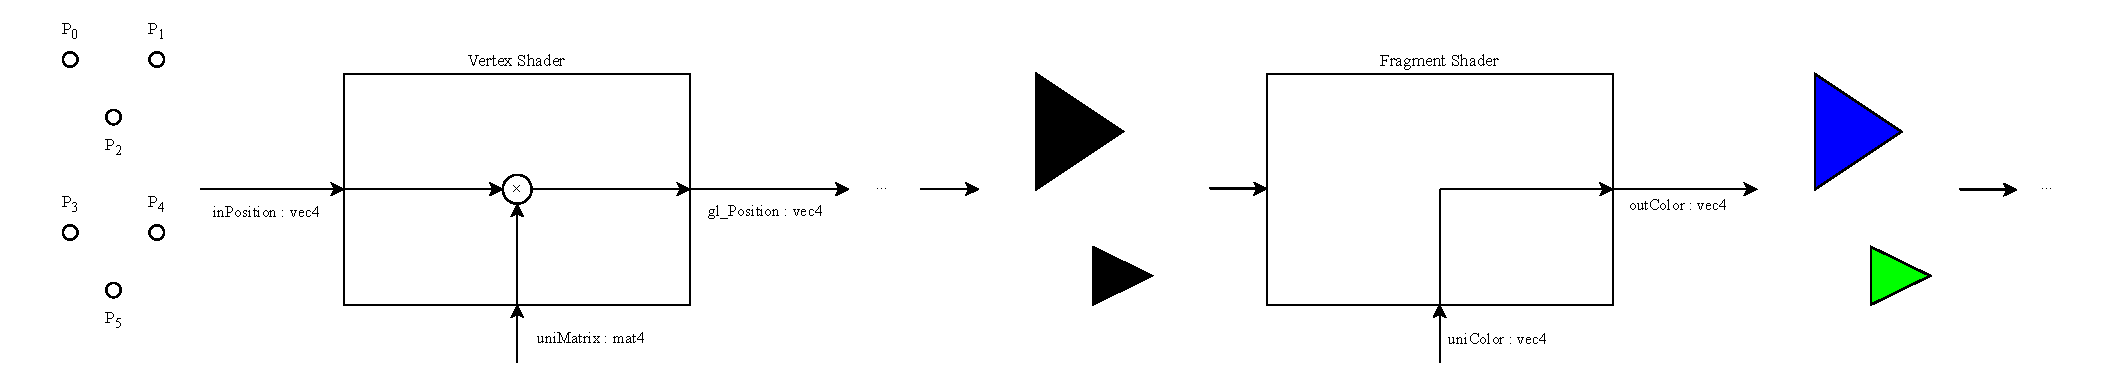
\includegraphics[width=\textwidth]{res/phase3/Shaders.pdf}
    \caption{Esquema dos \emph{shaders} desenvolvidos na \emph{pipeline} de renderização.}
\end{figure}

Como se pode observar, a única responsabilidade do \emph{shader} de vértices é multiplicar as
coordenadas das posições dos vértices que recebe por uma matriz de transformação passada numa
variável uniforme. Após o processamento dos vértices, dar-se-á o \emph{clipping}, a montagem das
primitivas, a divisão da perspetiva, a transformação pela \emph{viewport}, e a rasterização
\cite{vertex-post-processing}. Depois, para cada fragmento, o \emph{shader} de fragmentos será
invocado e, neste caso, atribuirá a todos os fragmentos das primitivas de um objeto a mesma cor,
passada como uma variável uniforme. Após a aplicação destes \emph{shaders} e algum processamento por
amostra, um objeto renderizado é colocado no \emph{framebuffer} para apresentação ao utilizador
\cite{per-sample-processing}. É de notar que a funcionalidade implementada por estes \emph{shaders}
é muito básica, apenas a necessária para o funcionamento correto da \texttt{engine} nesta terceira
fase do trabalho prático.

Após a criação dos \emph{shaders}, a \texttt{engine} carrega a cena e, para cada modelo, é criado um
\emph{Vertex Array Object} (VAO), algo que é obrigatório no \emph{core profile} do OpenGL. Com este
objeto vinculado, criam-se dois \emph{buffers}, um \texttt{GL\_ARRAY\_BUFFER}, no qual se armazenam
as posições dos vértices do modelo, e um \texttt{GL\_ELEMENT\_ARRAY\_BUFFER}, no qual se armazenam,
na forma de um \emph{array} de índices, a ordem em que estes vértices devem ser desenhados
\cite{glBufferData}. O uso de índices permite diminuir o tamanho dos modelos e tirar proveito da
cache de vértices da GPU. A figura abaixo mostra como estes três objetos estão relacionados:

\begin{figure}[H]
    \centering
    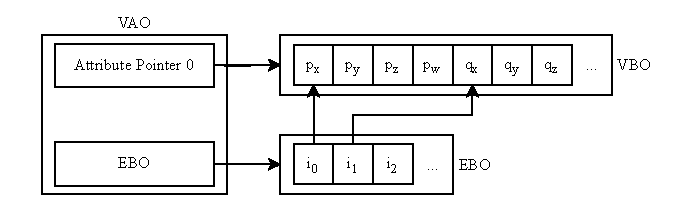
\includegraphics[width=\textwidth]{res/phase3/VAO.pdf}
    \caption{Organização do VAO, VBO, e EBO de um modelo.}
\end{figure}

Depois de criados estes objetos, para desenhar uma entidade na cena, basta vincular o seu VAO
correspondente e invocar a função \texttt{glDrawElements}.

O processo de envio de geometria para a GPU é semelhante para os eixos e para as representações
visuais das curvas de Catmull-Rom na cena. No entanto, não são criados \emph{arrays} de índices para
estes objetos, visto que não se espera que tenham vértices em duplicado. Então, a função usada para
desenhar estes objetos é \texttt{glDrawArrays}, e as primitivas são formadas com os vértices do VBO
pela ordem em que surgem no mesmo.

\subsection{Câmara em Terceira Pessoa}

\section{Resultados Obtidos}

\section{Conclusão e Trabalho Futuro}

\begingroup
\section{Bibliografia}
\renewcommand{\section}[2]{}

\begin{thebibliography}{9}
    \bibitem{wavefront-obj}
        ``Wavefront OBJ File Format Summary.'' FileFormat.Info. Accessed: Apr. 13, 2025. [Online.]
        Available: \url{https://www.fileformat.info/format/wavefrontobj/egff.htm}
    \bibitem{optimal-grid}
        ``Optimal Grid Rendering.'' Ignacio Castaño. Accessed: Apr. 14, 2025. [Online.] Available:
        \url{https://www.ludicon.com/castano/blog/2009/02/optimal-grid-rendering/}
    \bibitem{renderdoc}
        ``RenderDoc.'' RenderDoc Accessed: Apr. 14, 2025. [Online.] Available:
        \url{https://renderdoc.org/}
    \bibitem{vertex-post-processing}
        ``Vertex Post-Processing.'' OpenGL Wiki. Accessed: Apr. 13, 2025. [Online.] Available:
        \url{https://www.khronos.org/opengl/wiki/Vertex_Post-Processing}
    \bibitem{per-sample-processing}
        ``Per-Sample Processing.'' OpenGL Wiki. Accessed: Apr. 13, 2025. [Online.] Available:
        \url{https://www.khronos.org/opengl/wiki/Per-Sample_Processing}
    \bibitem{glBufferData}
        ``glBufferData.'' OpenGL 4.5 Reference Pages. Accessed: Apr. 15, 2025. [Online.] Available:
        \url{https://registry.khronos.org/OpenGL-Refpages/gl4/html/glBufferData.xhtml}
\end{thebibliography}
\endgroup

\end{document}
